\documentclass[tikz]{standalone}


\usetikzlibrary{shapes}
\usetikzlibrary{calc} 
\usetikzlibrary{positioning}


% This bascially automates a \newcommand{<name>}{} to ensure
% that a command with the given <name> does not already exist
\providecommand*{\pgfmathsetnewmacro}[2]{%
    \newcommand*{#1}{}% Error if already defined
    \pgfmathsetmacro{#1}{#2}%
}%


\begin{document}
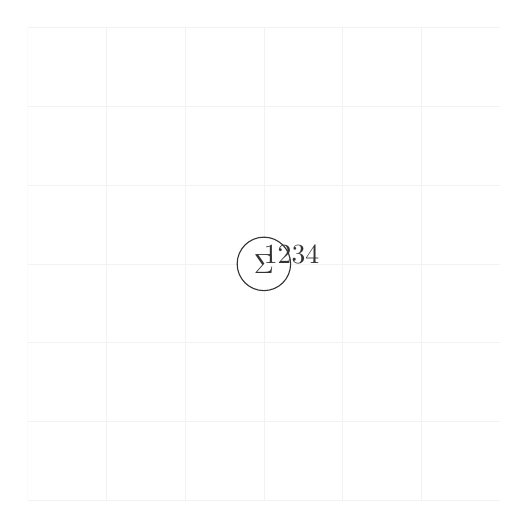
\begin{tikzpicture}[black!80]
    \pgfmathsetnewmacro{\bb}{3}
    \useasboundingbox[clip] (-\bb,-\bb) rectangle (\bb,\bb);


    \coordinate (O) at (0,0);

    \draw[help lines, opacity = 0.1] (-4,-4) grid (4,4);

    \begin{scope}[on grid]
        
        \node (O) at (0,0) [circle, draw, fill = white] {$\Sigma$};
              
        \foreach \node in {1, 2, 3, 4}{
            \node (I\node) [left = of O]  {$\node$};
        }
        
    
    \end{scope}
        

    
    
    
\end{tikzpicture}
\end{document}